\subsection{MV*-Architekturmuster}
Häufig unterstützen Webframeworks, aber auch diverse Content Management-Systeme, verschiedene Architekturmuster, um die Entwicklung von Webanwendungen modularer zu gestalten. Der Gedanke dabei ist es, den Quellcode zum Beispiel in Logik und Präsentation aufzuteilen. So ist der Code für Entwickler leichter zu warten, die Testbarkeit verbessert sich und es ergeben sich wiederverwendbare Codestücke \cite[S. 34]{ste15}. \\
Eines dieser Entwurfsmuster ist das \ac{mvc}. Dieses besteht aus drei Komponenten. Wie diese interagieren, beschreibt \autoref{img:mvc}.

\begin{figure}[H]
	\begin{center}
		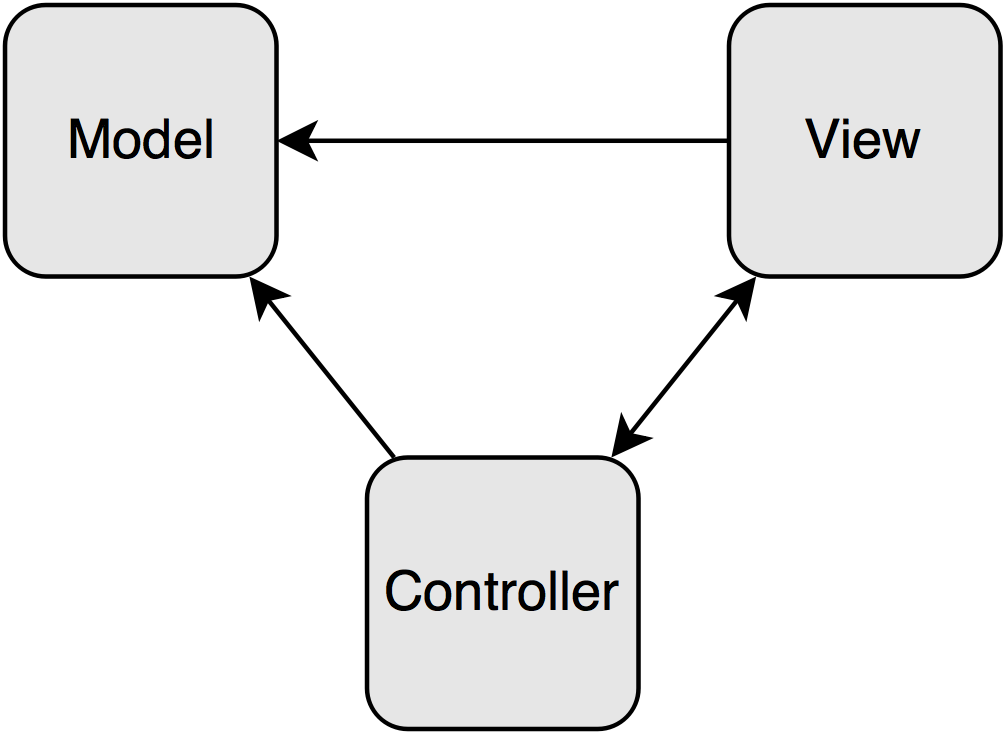
\includegraphics[width=.6\textwidth]{mvc.png}
		\caption{MVC-Muster}
		\label{img:mvc}
	\end{center}
\end{figure}

Die Model-Komponente beinhaltet die darzustellenden Daten. In der View-Komponente wird beschrieben, wie die Daten darzustellen sind. Die Controller-Komponente regiert auf Benutzeraktionen und beeinflusst die Darstellung der View und die Daten des Models. Zudem können beim \ac{mvc} komplexere Views in mehrere einzelne Views aufgeteilt und ineinander verschaltet werden \cite[S. 5 ff.]{gof}.

Als weiteres Entwurfsmuster ist das \ac{mvvm} zu nennen. Model und View entsprechen dem des \ac{mvc}-Musters. Anstelle eines Controllers wird hier aber ein View-Model eingesetzt. Hier wird die Logik der Bedienoberfläche (View) beschrieben und referenziert zu den Daten (Model) \cite[S. 40]{mvvm}, vergleiche \autoref{img:mvvm}. Im Gegensatz zum Controller im \ac{mvc}-Muster besitzt das View-Model hier keinerlei Informationen über die View. Dies erleichtert den Austausch der View und erlaubt, dass sich mehrere Views auf ein View-Model beziehen.

\begin{figure}[H]
	\begin{center}
		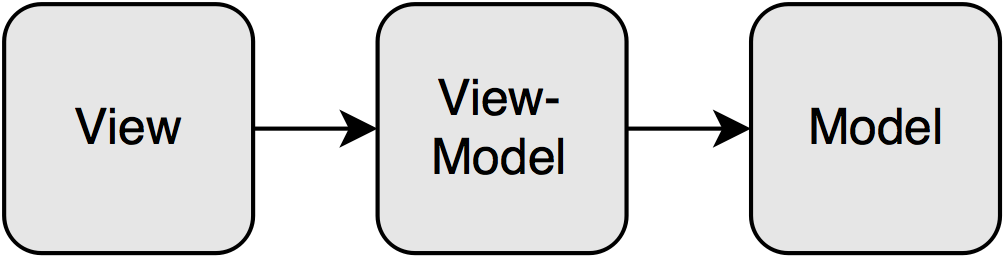
\includegraphics[width=.6\textwidth]{mvvm.png}
		\caption{MVVM-Muster}
		\label{img:mvvm}
	\end{center}
\end{figure}

Bei MV*-Architekturmustern wird die View häufig durch ein oder mehrere Templates (Vorlagen) beschrieben. Im Zusammenhang mit MV* ist ein Template eine Vorlage für das Aussehen einer Webseite, in dem wiederkehrende Elemente definiert werden. Diese werden für gewöhnlich in separaten Dateien gespeichert und mit Platzhaltern und einer einfachen Logik versehen. Anhand der Daten des Models und ggf. weiterer Variablen werden die Platzhalter gefüllt und so ein HTML-Dokument erstellt, das dem Clienten zugeschickt wird. Die semantische Darstellung der Platzhalter und des Logikflusses ist von der verwendeten Templatesprache abhängig \cite[S. 37]{newman2008django}.